\documentclass[a4paper,UKenglish,cleveref, autoref, thm-restate]{lipics-v2021}
\usepackage{subfiles}

% Use the postscript times font!
\usepackage{times}
\usepackage{soul}
\usepackage{multirow}
\usepackage{url}
\usepackage{hyperref}
\usepackage[utf8]{inputenc}
%\usepackage[small]{caption}
\usepackage{graphicx}
\usepackage{amsmath}
\usepackage{amsthm}
\usepackage{booktabs}
% \usepackage{algorithmic} % Conflicting with algpseudocode
%\usepackage[switch]{lineno}
\usepackage{listings}
\usepackage{xcolor}
\usepackage{algorithm}
\usepackage{algpseudocode}
\usepackage[dvipsnames]{xcolor}

% comments
\usepackage{color}
\definecolor{mygreen}{rgb}{0,0.6,0}
\definecolor{darkGreen}{rgb}{0,0.4,0}

\newcommand{\crc}[1]{\textcolor{red}{ #1}}
\newcommand{\crcf}[1]{\textcolor{blue}{ #1}}

%\authorrunning{Anonymous}
%\hideLIPIcs
\lstset{
  basicstyle=\scriptsize\ttfamily,
  columns=fullflexible, keepspaces=true,
  tabsize=2, stepnumber=1,
  numbers=left,
  captionpos=b,
  xleftmargin=5mm
}

\keywords{Constraint modelling, algorithm selection, machine learning, constraint solvers.}

\ccsdesc{Computing methodologies~Artificial intelligence}

\title{Using Weisfeiler-Leman Features for Algorithm Selection in Constraint Optimisation}

\titlerunning{Using Weisfeiler-Leman Features for Algorithm Selection in Constraint Optimisation}

\author{Anonymus}{Anonymus}{Anonymus}{}{}

\authorrunning{Anonymus}

\Copyright{Anonymus}

\begin{document}


\maketitle

\begin{abstract}
We have new features and they are decent enough.

\end{abstract}

\section{Introduction}
Algorithm Selection is a critical component in the efficient execution of Constraint Programming models, as solver performance varies significantly across different problem instances. Traditional feature extraction methodologies, such as \texttt{fzn2feat}, primarily rely on instance-level statistics that often fail to capture the underlying latent structure and the complex interconnections between variables. While graph-based representations are designed to capture these structural nuances, they are typically coupled with deep neural networks that require substantial computational overhead. This creates a representational gap: non-neural machine learning techniques remain largely ``structure-blind,'' while structure-aware models are often too expensive for practical deployment.

This paper proposes a novel methodology to bridge this gap by implementing a graph conversion algorithm compatible with both classical and deep machine learning paradigms. Our approach utilizes Weisfeiler-Lehman graph kernels to generate robust representations of problem instances. The primary innovation is the introduction of a cut-based representation, which explicitly models structural partitions to provide a more nuanced predictive signal than standard graph features.

To evaluate the efficacy of these features, we constructed three distinct algorithm selection tasks using instances from the 2023, 2024, and 2025 MiniZinc Challenges. Experimental results across Support Vector Machines, Random Forests, and Multi-Layer Perceptrons demonstrate that our features outperform \texttt{fzn2feat} on two out of three tasks, often. Notably, the \texttt{WLc} features often achieved statistically significant improvements ($p < 0.05$), while never performing statistically worse than \texttt{fzn2feat} in any configuration. Our work effectively demonstrates that graph-based structural information can be leveraged to enhance traditional machine learning architectures, ensuring performance gains that are robust across diverse algorithmic structures.
\section{Background}
This section provides the theoretical foundation for this work while excluding Graph-based representations of constraint problems as we will discuss them in Section \ref{sec:conversion}.

\subsection{Combinatorial Optimisation}
Constraint Programming (CP) \cite{rossi2006handbook} is a paradigm for solving combinatorial optimization problems (COPs) by defining them via variables, domains, and constraints. Unlike other combinatorial solvers, CP utilizes global constraints (such as \textit{all-different}, \textit{cumulative}, or \textit{circuit}) which capture complex substructures. These constraints use specialized filtering algorithms to prune the search space through propagation, enabling more efficient modeling and solving.

Constraint solvers navigate the solution space using techniques like constraint propagation \cite{bessiere2006constraint}, branch and bound \cite{boyd2007branch}, and conflict-driven clause learning (CDCL) \cite{marques2009conflict}. Given that COPs are often NP-hard \cite{Papadimitriou_book}, parallelization is frequently employed to speed up the computation. This typically follows two patterns: (i) the job-splitting approach, which parallelizes a single solver's strategy, and (ii) the portfolio approach, which runs multiple solvers with different strategies simultaneously \cite{paper_amai}. Comprehensive reviews for parallelizing these specific techniques are available in \cite{gent2018review, crainic2006parallel, martins2012overview}.

\subsection{Algorithm Selection}
Algorithm Selection (AS) involves identifying the most suitable algorithm for a specific problem instance to optimize metrics like computational efficiency or accuracy. This process is necessitated by the No Free Lunch theorem \cite{wolpert1997no}, which states that no single algorithm is universally superior. In the SAT domain, SATZilla \cite{xu2012satzilla2012} uses AS to manage solver portfolios. In CP, approaches like CPHydra \cite{bridge2012case} and SUNNY \cite{amadini2014sunny} utilize $k$-nearest neighbors (k-NN) to generate instance-specific solver schedules.

\subsection{Feature Extraction on Graphs}
Feature extraction transforms graph-structured data into fixed-dimensional vector spaces \cite{graphkernels}. Classic methods rely on graph-theoretical metrics to describe structural properties.

Node-level features describe a node's topological importance. Common metrics include Degree Centrality, Clustering Coefficient \cite{watts1998collective}, and Betweenness or Closeness Centrality \cite{newman2010network}. Edge-level features are primarily used for link prediction and node proximity. These include Common Neighbors, the Jaccard Coefficient, the Adamic-Adar Index (which weights neighbors by their rarity) \cite{adamic2003friends}, and the Katz Index \cite{Luce_Perry_1949}.

Graph-level features are often extracted via kernels that compute similarity as a scalar product between two graphs $G_1$ and $G_2$. 
\begin{itemize}
    \item \textbf{Weisfeiler-Lehman (WL) Kernel} \cite{shervashidze2011weisfeiler}: Iteratively relabels nodes based on neighbor signatures (see Section \ref{sec:wl}).
    \item \textbf{Graphlet Kernel} \cite{graphkernels}: Counts small, non-isomorphic subgraphs.
    \item \textbf{Random Walk Kernel} \cite{vishwanathan2010graph}: Compares graphs based on matching paths.
\end{itemize}
WL-based features are widely used in cheminformatics and computer vision \cite{young2022literature, simonovsky2017dynamic}  as well as in neighbour fields like planning \cite{chen2024return}. Furthermore, the message-passing mechanism in Graph Neural Networks is fundamentally inspired by the WL algorithm \cite{Xuetal2018, morris2023weisfeiler}.
\section{Graph Conversion}\label{sec:conversion}

As stated in Section \ref{sec:graph-representation}, many different approaches for graph conversions have been proposed. Our approach is inspired by that of Boisvert et al. \cite{boisvert2024towards}, but, unlike them, we do not include domain values in our representation. We decided to exclude domain values for practical reasons: the argument of Boisvert et al. to include them, lies on the injection of the conversion, without domain values two instances could end up being mapped into the same graph. While true, our primary objective is to use the features for algorithm selection and, as an example, an instance from the 2025 Minizinc challenge\footnote{\url{https://www.minizinc.org/challenge/2025/results/}} (coming from the cgt problem with instance name cgt\_12\_h27\_r0.05\_s0.5\_3) had an objective function with a domain between -1.932.060 and 1.714.644, resulting in 3.646.705 total possible values just for one domain. The full instance would also require adding also other variables and their domains as well as constraints and operators. A graph with this many nodes would be intractable for our purposes. Furthermore, our graphs are directed instead of undirected. This choice allow us to have shallow graphs with small diameters making it possible to convey all the information with a limited amount of aggregation steps. We have decided to use Boisvert et al.'s syntax tree-like representation as it allows us to decompose complex constraints into simpler elements that could be reused in different constraints with similar meanings.

In more details, we define five types of nodes:
\begin{itemize}
    \item \textbf{Variable nodes}: representing the variables of the problem. 
    \item \textbf{Solution node}: a single node for each problem that represents the type of problem (Minimisation, Maximisation or Satisfaction).
    \item \textbf{Parameter/Literal nodes}: representing the literal values of the problem (e.g. 1, 2, True, False, etc.).
    \item \textbf{Operator nodes}: representing arithmetic and functional operations between variables, parameters and other operators (e.g. $+$, $\times$, $\div$ etc.) Operator nodes have a sub-category for the type of operator represented.
    \item \textbf{Constraint nodes}: representing relational predicates (e.g. $=$, $\neq$, $<$, $\leq$), logical operations (e.g. $\wedge$, $\vee$, $\neg$), and global constraints (e.g. \texttt{all\_different}, \texttt{table}). Constraint nodes also have a sub-category for the type of constraint the node represents. 
\end{itemize}
All node and sub-node types we have defined for the conversion from FlatZinc can be seen in the Appendix \ref{sec:node-types}.

As previously mentioned, edges between nodes are directed: variables and parameter nodes have no incoming nodes and only point to the operators or constraints they take part in. There is only one exception: for optimisation problems, the variable containing the objective value to optimise has an incoming edge from the Solution node. Operator nodes can have both incoming and outgoing edges. Incoming edges come from variables, parameters and other operators that take part in the operation. Outgoing edges go to other operator nodes or to constraint nodes. Constraint nodes can also have edges to other constraint nodes when they appear as a sub-expression to other constraints. As an example, the expression $(x = 3) \wedge (y \neq 5)$, will have three constraint nodes ($=$, $\wedge$ and $\neq$) with $=$ and $\neq$ having exiting edges to $\wedge$.

Edges are typed as well; in particular, there are three types of edges: 
\begin{itemize}
    \item \textbf{Lead edges}: used to connect variables, parameters and operators to operators and constraints for which the order of the operands does not matter (e.g. sum or equality). Lead Edges are also used for variables, parameters and operators that fall on the left side of an operation or constraint where the order of the operands matters (e.g. subtraction or strictly less than). Lead edges are also used to connect the solution node to the objective variable in optimisation problems.
    \item \textbf{Trailing edges}: Used to connect variables, parameters and operators to operators and constraints for which the order of the operands matters and the operands fall on the right side of the operation.
    \item \textbf{Global edges}: Used to connect variables and parameters to global constraints. This helps to distinguish normal connections from normal and global constraints.
\end{itemize}

\begin{figure}[ht]
    \centering
    \begin{subfigure}[c]{.45\textwidth}
        \begin{lstlisting}
var int x;
var int y;
constraint 3*x <= y;
constraint y < 10;
all_different([x, y]);
solve maximise x;\end{lstlisting}
    \end{subfigure}%
    \begin{subfigure}[c]{.45\textwidth}
        \centering
        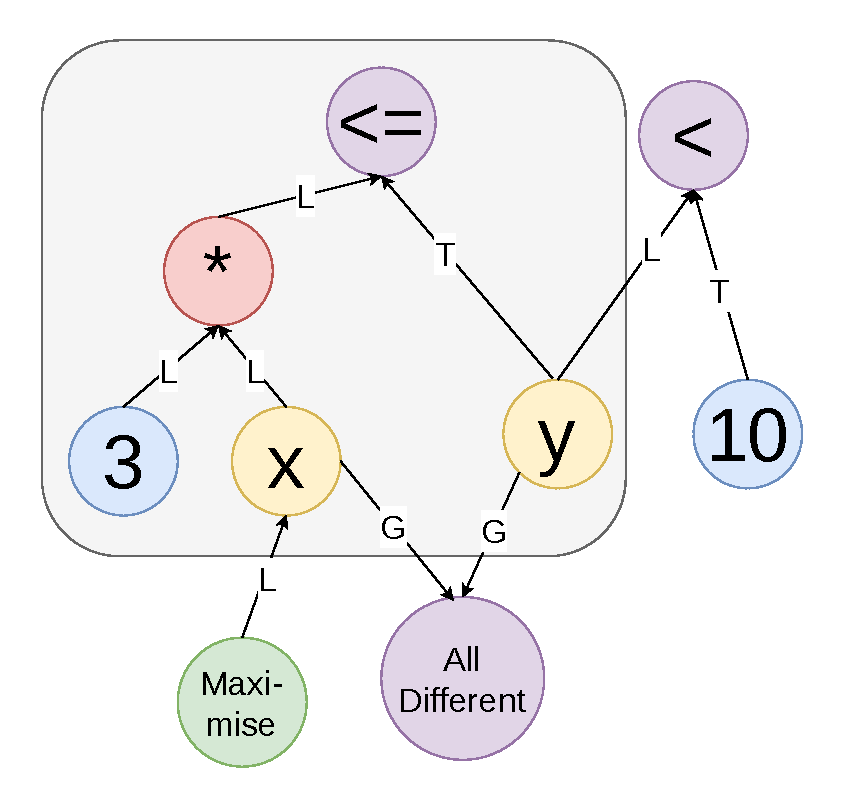
\includegraphics[width=.9\textwidth]{figures/graph.drawio.pdf}
    \end{subfigure}
    \caption{Conversion of a constraint model (left) to a graph (right). Variables in yellow, Parameters in blue, Operators in red, Constraints in purple, and Solve in green. The area in gray represents the constraint \texttt{3*x <= y}. Lead edges are labelled as L, Trailing as T and Global as G.}
    \label{fig:conversion}
\end{figure}

Figure \ref{fig:conversion} shows an example of how a simple constraint model can be converted using our conversion methodology.
\section{Extracting Features Using The Weisfeiler-Leman Algorithm}\label{sec:feature_Extraction}
Once we have defined how to convert any instance to a graph, we can use the WL algorithm to extract features from the graphs. 

\begin{figure}[t]
    \centering
    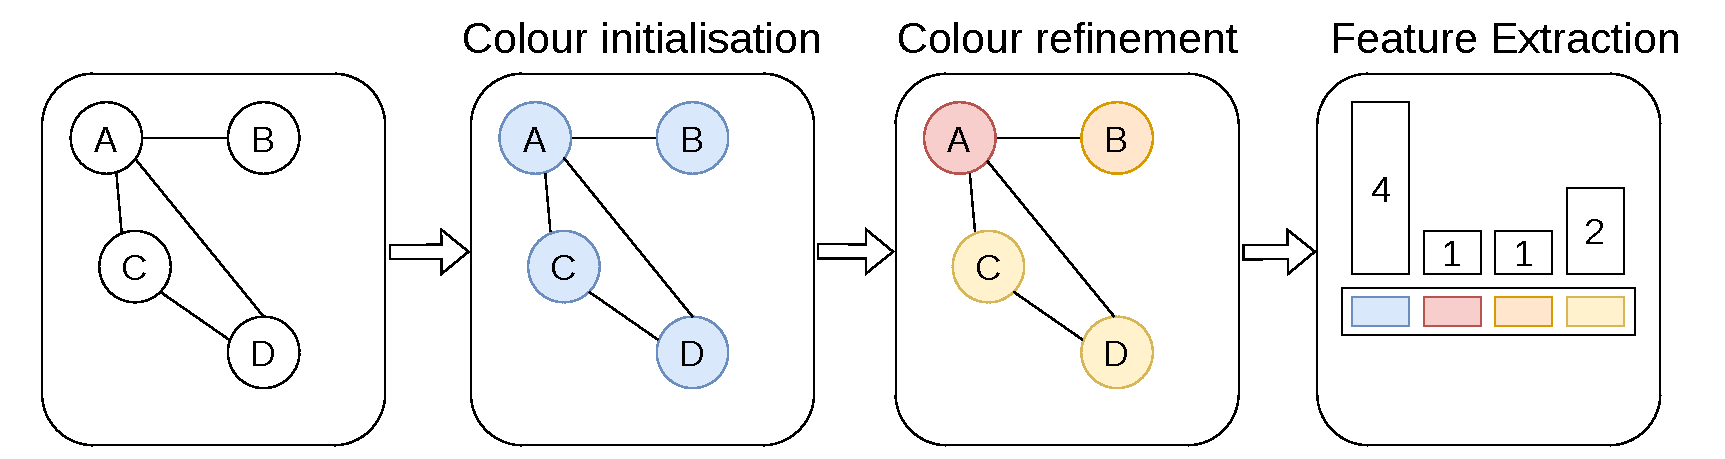
\includegraphics[width=.8\textwidth]{figures/wl.drawio.pdf}
    \caption{Feature extraction process using the WL algorithm on a simple, undirected graph. The colour refinement is executed only once. At first, all nodes get the same colour, then node A aggregates its colour (blue) with its 3 neighbours' colours (blue), getting, as a result, (blue, blue,blue,blue). This produces a new colour, red. C and D, having only two neighbours, get, as aggregation (blue, blue,blue), resulting in the new colour yellow and, finally, node B, having only one neighbour, aggregates to (blue, blue), getting as new colour orange. In the final steps, we count the number of occurrences of each colour, and we get 3 blues from the original initialisation and 1 red, 1 orange and 2 yellow after the first aggregation step.}
    \label{fig:wl-feature-exec}
\end{figure}

\subsection{WL For Feature Extraction}\label{sec:wl-feature_Extraction}
To use the WL algorithm for feature extraction, we repeat the colour refinement process for a pre-defined number of steps on a single graph, then we extract features by creating a histogram where, for each colour, we count the number of occurrences. Then, the final feature vector is created by concatenating the histograms after each iteration. A depiction of the execution of the WL algorithm for feature extraction (with one aggregation step) can be seen in Figure \ref{fig:wl-feature-exec}.

Note that while the standard WL feature extraction process typically concatenates histograms from all iterations, we deliberately utilise only the final histogram. This decision is informed by several theoretical and practical considerations specific to our domain.

First, from a theoretical perspective, the final iteration's labels represent the most refined partition of the graph's nodes. As demonstrated in the analysis of Graph Isomorphism Networks \cite{Xuetal2018}, the final state of a message-passing scheme (given an injective aggregation function) effectively encodes the full subtree structure. In our discrete WL implementation, the final labels serve as a compressed representation that implicitly preserves the structural history of previous iterations.

Furthermore, the specific topology of our data justifies this approach. The extracted graphs are characterised by a shallow diameter and directed edges, which significantly limit the depth of information flow. In such instances, the WL process converges rapidly as nodes quickly incorporate all available predecessors' information. Our empirical analysis (in Appendix \ref{sec:ablation-study}) across three distinct tasks and three different ML models confirmed this; we found no statistically significant difference in performance between concatenated features and the single-histogram approach. Consequently, we prioritise the latter.

\subsection{Enhancing Features' Expressiveness}
The standard WL features are designed for graphs without any edge or node information. However, in our case, we have both node and edge-level information we can use to better represent the input graph. For this reason, inspired by previous works \cite{Togninalli2019-qa},  we include two extensions to the base algorithm:
\begin{itemize}
    \item \textbf{Node-information extension}: To add node information into the extraction process, we can initialise the node colour with the hash of its type + subtype (e.g. a \texttt{Variable node} and a \texttt{Sum node} will be initialised with different colours). Formally, $c^{(0)}(v) \leftarrow \text{HASH}(\text{type}(v) \ || \ \text{subtype}(v))$ where $||$ denotes string concatenation.
    \item \textbf{Edge-information extension}: To add edge information into the extraction process, we can concatenate the edge type to the node colour during the aggregation step (e.g. in the example of Figure \ref{fig:wl-feature-exec}, if Node B was connected to node A via a Leading edge, the aggregation of node B would be: (blue, blue-L)). Formally, assuming a directed graph where edges flow towards $v$, its multiset update becomes $M(v) \leftarrow \{\!\!\{c^{(t-1)}(w) \ || \ \text{type}(w, v) \mid (w,v) \in E\}\!\!\}$.
\end{itemize}
Finally, we can use the fact that our graphs are directed and only update a node colour based on its incoming neighbours.

Using these extensions, we can now define four types of features: (i) \texttt{WL}, standard WL features without node or edge information, (ii) \texttt{WLn}, WL features enhanced via node-information extensions, (iii) \texttt{WLe},  WL features enhanced via edge-information extensions, and (iv) \texttt{WLne}, WL features enhanced with both edge and node-information. 

\subsection{The ``Cut'' Trick}
In the WL algorithm, the colour of a node is highly dependent on its degree, and two nodes with different degrees, even when sharing the same original colour and the same type of neighbour nodes, will end up with different colours. This can be problematic for nodes representing operators and constraints where the number of connected sub-elements can vary. As an example, let's examine the \texttt{all\_different} global constraint: using the standard algorithm, \texttt{all\_different([v1, v2, v3])} will get a totally different and uncorrelated colour to \texttt{all\_different([v1, v2])} solely due to its degree. In practice, while preserving some differences between the two constraints, we would still capture the fact that they are pretty similar.

To achieve this, we can virtually ``cut'' the connections between the nodes representing constraints and operators with a variable number of operands in them. We will refer to these nodes as cut nodes. In practice, during the aggregation steps, the cut nodes will not be updated since their incoming connections will be ignored. However, the cut nodes will still contribute to the update of the nodes they are connected to via their outgoing edges. All cut nodes can be seen in Appendix \ref{sec:node-types}. 

After the aggregation steps have been completed, each cut node's colour can be updated by aggregating it with the set (not multiset) comprised of all its connected, original node colours. By using a set rather than a multiset, nodes with the same type of incoming nodes will receive the same colour, independent of their degree.

At this stage, we can correctly capture the fact that two constraints with the same type of connected nodes but different degrees have the same colour; however, we are completely missing any information regarding the degree of a node, information that we would still like to capture. To do so, we can add extra features after the colour histogram. Specifically, from each cut node, we can generate node pairs comprising the cut node and its incoming neighbours. Thus, each cut of degree $n$ will generate $n$ pairs. After having generated all the pairs, we count the occurrence of each pair in a graph to generate a histogram of pairs and concatenate it to the histogram of colours.

The cut trick can only be applied when node information is present, thus, only to \texttt{WLn} and \texttt{WLne} features. We will call the features where the cut trick is applied \texttt{WLc-n} if only the cut is applied to \texttt{WLn} features and \texttt{WLc-ne} if the cut is applied to \texttt{WLne}. A formalisation of the \texttt{WLc-n} features can be seen in Algorithm \ref{alg:wl-cut}, and a graphical depiction of how the cut trick is applied can be seen in Figure \ref{fig:cut-trick}.

\begin{algorithm}[ht]
\scriptsize
\caption{\texttt{WLc-n} Algorithm for Feature Extraction. The \texttt{WLc-ne} version will be different only in the aggregation step, where the edge information will also be included.}
\label{alg:wl-cut}
\begin{algorithmic}[1]
\Require Graph $G = (V, E)$, iterations $T$, subset $V_{cut} \subseteq V$ of cut nodes
\Ensure Feature histograms of colours and pairs
\State \textbf{Initialisation:} $c^{(0)}(v) \leftarrow \text{HASH}(\text{type}(v) \,||\, \text{subtype}(v))$ for all $v \in V$
\State $t \leftarrow 0$
\Repeat
    \State $t \leftarrow t + 1$
    \For{each node $v \in V$}
        \If{$v \notin V_{cut}$}
            \State $M(v) \leftarrow \{\!\!\{c^{(t-1)}(w) \mid (w,v) \in E\}\!\!\}$
            \State $c^{(t)}(v) \leftarrow \text{HASH}(c^{(t-1)}(v), \text{sort}(M(v)))$
        \EndIf
    \EndFor
\Until{$t = T$}
\State $Pairs \leftarrow \{\!\!\{\}\!\!\}$ \Comment{Initialize multiset for pairs histogram}
\For{each node $v \in V_{cut}$}
    \State $S(v) \leftarrow \{ c^{(0)}(w) \mid (w,v) \in E \}$ \Comment{Set of initial colours (types) of incoming neighbours}
    \State $c^{(final)}(v) \leftarrow \text{HASH}(c^{(T)}(v), \text{sort}(S(v)))$
    \For{each node $w$ where $(w,v) \in E$}
        \State $Pairs \leftarrow Pairs \cup \{\!\!\{ (c^{(0)}(w), c^{(0)}(v)) \}\!\!\}$
    \EndFor
\EndFor
\State $c^{(final)}(v) \leftarrow c^{(T)}(v)$ for all $v \in V \setminus V_{cut}$
\State \Return $\text{Histogram}(c^{(final)}) \cup \text{Histogram}(Pairs)$
\end{algorithmic}
\end{algorithm}

\begin{figure}[t]
    \centering
    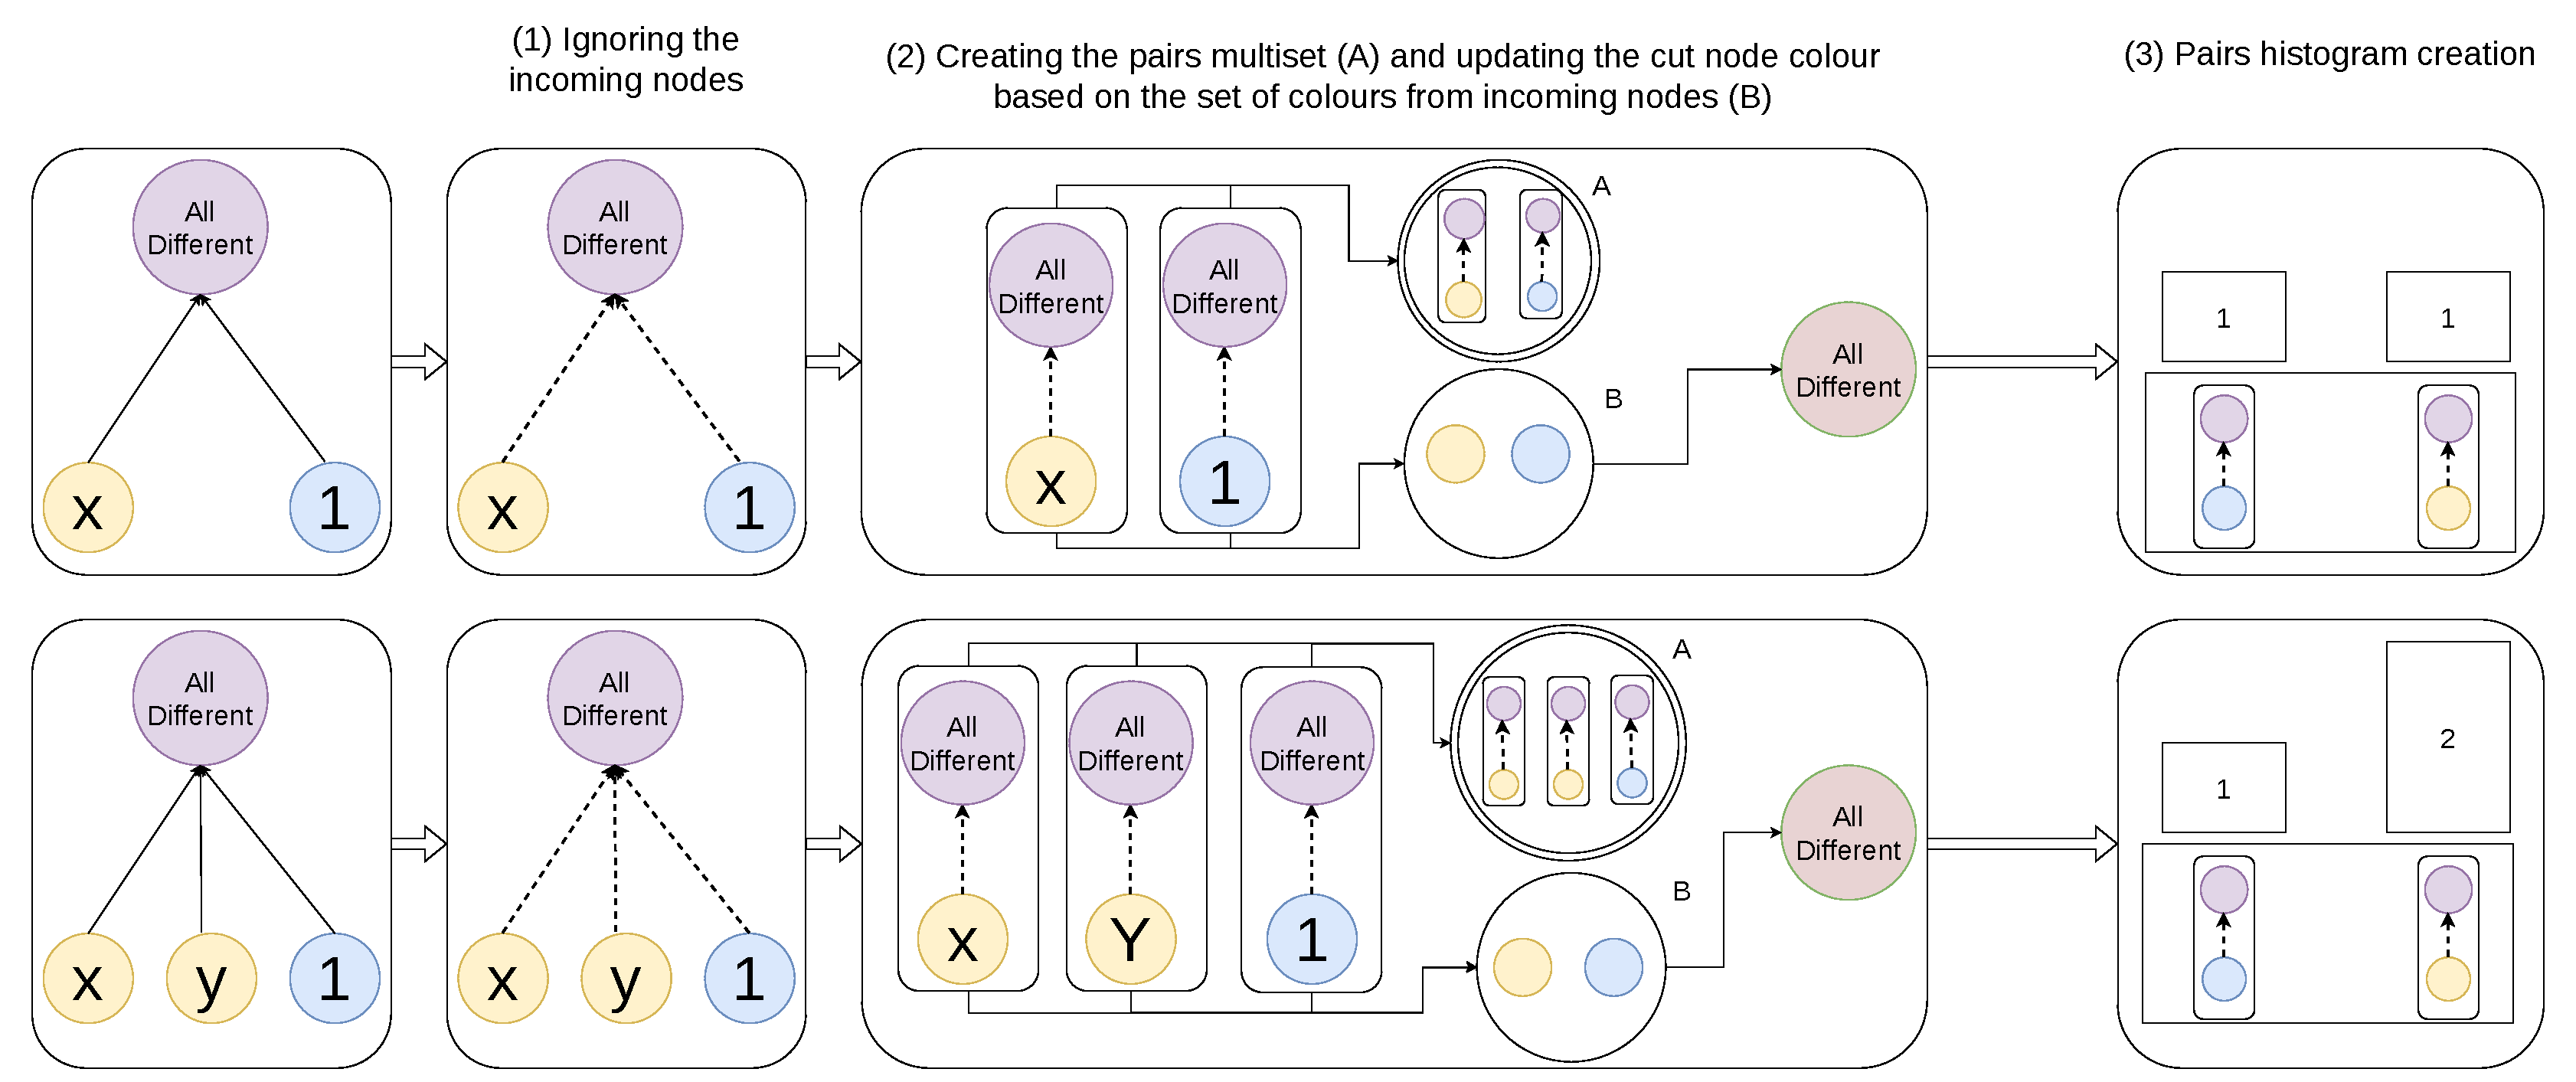
\includegraphics[width=.87\linewidth]{figures/wlc.drawio}
    \caption{Application of the cut trick on two occurrences of the \texttt{all\_different} constraint (top and bottom). Constraint nodes are in purple, variable nodes in yellow and parameter nodes in blue. First, cut nodes do not perform the normal WL aggregation steps (1), then we generate all pairs and update the colour of the \texttt{all\_different} node by aggregating it with the set of all types of node with incoming edges (2) and then we generate the pairs histogram by counting all the occurrences of the pairs (3). In this example, since both constraints share the same type of incoming nodes, they will be coloured in the same way. However, having a different node degree will result in a different pair histogram.}
    \label{fig:cut-trick}
\end{figure}

\subsection{Features, Characteristics, and Normalisation} \label{sec:feature_characteristics}
As a consequence of our design choices, especially of having directed graphs, the extracted features have emerging properties that are worth noting. In particular, since variable and parameter edges have no incoming node (but for the variable connected to the objective function), the colours of those values never get updated. Thus, one value in the final feature set would represent the number of variables in the graph, and another the number of parameters in the graph.

To give some extra information about variables and parameters in the graph, besides their total count, we decided to add two extra features, one representing the average number of constraints/operators a variable takes part in and one representing the same but for parameters.

Also, due to the direct nature of our graphs, most paths in the graph are quite shallow, especially after the cut. As an example, in the \texttt{x + 3 = y} constraint, we will have 2 variable nodes, (\texttt{x, y}), one parameter node (\texttt{3}), one operator node (\texttt{+}) and one constraint node (\texttt{=}). The operator node can be updated only once since the values of the parameter and variable nodes connected to it will never get updated. At the same time, the value of the constraint node can be updated at most twice: once at the first step when it aggregates with the original \texttt{+} and \texttt{y} colours and once at the second step when it aggregates with the updated \texttt{+} colour and the original, unmodified \texttt{y} colour. For a deeper discussion on the depth of the produced graphs, see Appendix \ref{sec:graph-depth}. 

Global constraints are always terminal nodes without any outgoing nodes; thus, as a consequence, updating them only once, at the end of the standard WL steps, will result in the same output as updating them during the standard WL steps.



Finally, once the final histograms are extracted from the graphs, we need to normalise the features. This is a necessary step since the values in the histograms will grow proportionally to the size of the graph. Thus, if not normalised, the produced histograms will be comparable only with those produced by graphs of the same size, making it impossible to generalise.

We decided to normalise the colour histograms by dividing each value in the histogram by the total count of nodes. Similarly, the pairs histogram is normalised by the total pairs count. This normalisation step will generate a final feature set with values always smaller than or equal to 1.

\subsection{Train and Test Feature Extraction Process}
During the extraction process, different graphs will generate different colours, and only a subset of those will be shared between different graphs. This will result in feature sets with different histogram sizes and with different colours in them. To train an ML model, we need to standardise the histograms, making them share the same colours. To do so, we can collect all colours from all histograms and add a 0 coefficient to all colours missing in a histogram. 

During testing, if we encounter a new colour not present in the training data, we simply discard it and ignore the update.
\section{Experimental Results}
To test our methodology, we have implemented the graph conversion algorithm on top of the Flatzinc modelling language. We have then taken the instances from three Minizinc challenges (2023, 2024, and 2025), for a total of 300 instances and designed three different algorithm selection tasks around it: (i) algorithm selection based on the Borda count score on three solvers where the objective is to maximise the score, (ii) the same algorithm selection task but where the objective is to maximise the prediction accuracy and (iii) running a solver in its sequential and parallel version, we seek to predict if the parallel solver will meaningfully increase the performance with respect to the sequential version. The evaluation metrics will be predictive accuracy. 

Each task will be compared against a baseline and the fzn2feat features: a feature set specifically designed for algorithm selection tasks for constraint programming. Due to the shallow depth of our graphs, we decided to test \texttt{WL}-based features with one or two aggregation steps.

For each task, we trained three different ML models: (i) Support Vector Machine (SVM), (ii) Random Forest and (iii) a simple, three layer, multi-layer-perceptron (MLP). And the training process followed a four-steps pipeline:
\begin{enumerate}
    \item Perform grid search on a predefined set of hyperparameter configurations and score each hyperparameter configuration based on the mean 5-fold cross-validation score.
    \item Select the hyperparameter configuration with the best score. Ties are broken by selecting the hyperparameter configuration with the lowest chance of overfitting:
    \begin{itemize}
        \item Lowest regularisation parameter, gamma and using the rbf kernel for SVM.
        \item Smallest number of trees and depth for Random Forest.
        \item Lowest number of training steps and smallest alpha for MLP.
    \end{itemize}
    \item Test the performance of the best configuration on a range of smaller features set obtained by applying PCA decomposition on the original features set. The tested values are in the range $[20, \min(\text{n\_features},\text{n\_training-datapoints})[$.
    \item Select the feature set with the highest score between those obtained by applying PCA decomposition and the original one.
\end{enumerate}

\subsection{Borda Count Score Maximisation}
In this task, we compared three sequential solvers on the 300 instances. The solvers were run without forcing them to follow the search annotations on a very old CPU (fill in) for a total of 20 minutes. On each instance, solvers have been scored based on the same borda count scoring strategy followed by the Minizinc challenge.\footnote{https://www.minizinc.org/challenge/2025/} 
The task has been modeled as a classification task where the prediction label corresponded to the solver with the highest score. Ties have been broken by assigning the label to the solver with the highest overall score. 
The three solver we selected are \texttt{Or-Tools}, \texttt{Chuffed} and \texttt{Cplex}. From the final dataset, we removed one instance which was trivially unsat (and from which it was impossible to extract features) and all instances where no solver ever found a solution. In the end, the final dataset was composed of 289 instances. We performed 5-fold cross-validation using a stratify strategy repeating the split 10 times with different random seeds for a total of 50 test. The train-test split was performed using Scikit-learn StratifiedKFold function\footnote{https://scikit-learn.org/stable/modules/generated/sklearn.model\_selection.StratifiedKFold.html} where the stratification was performed on the gap between the virtual best score (the maximum theoretical score obtainable) and the worse possible score. 


\bibliographystyle{plain}
\bibliography{references}


\end{document}
